\documentclass[a4paper,oneside]{ltjsarticle}
\usepackage[hiragino-pron]{luatexja-preset}
\usepackage{url}
\usepackage{amsmath,amssymb}
\usepackage{tikz}
\usepackage{bussproofs}
\usepackage{bcprules}
\usetikzlibrary{positioning,arrows,shapes,chains}
\usepackage{listings}
\lstset{%
	float=hbp,
	basicstyle=\ttfamily,
	numberstyle=\ttfamily\footnotesize,
	identifierstyle=,
	columns=flexible,
	tabsize=2,
	frame=single,
	extendedchars=true,
	inputencoding=utf8x,
	showspaces=false,
	showstringspaces=false,
	numbers=left,
	breaklines=true,
	breakautoindent=true,
	captionpos=t,
}
\title{AT-TaPL 4: Typed Assembly Language pt.1}
\author{河原 悟}
\begin{document}
\maketitle
P142〜

\setcounter{section}{-1}
\section{introduction}
適当に引っ張ってきたコードは正しく動くのか?
\begin{itemize}
	\item \textit{proof-carrying code(PCC)} by Necula amd Lee

		コードの性質の証明のチェックが簡単できて、proof-checking engineが小さい
\end{itemize}

PCCをうまく使っていくために、以下の問題を解決したい:

\begin{enumerate}
	\item コードが満たすべき性質とは?
	\item コードが満たすべき性質の証明をプログラマーはどう作るか?
\end{enumerate}

1. は文脈やアプリケーションに依存し、2. は自動的にはできない。ではどうするか?

\textit{type-preserving} compilationをベースにしたアプローチを考えてみる。
コードが満たすべき性質として型安全であることにフォーカスする。

この方法論では、コンパイルのプロセスとして型付きマシンコードにコンパイルされる型付きの中間言語をデザインする必要がある。
\begin{figure}[ht]
	\centering
	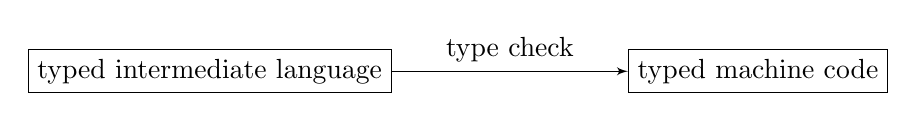
\begin{tikzpicture}
		\node[draw] (A) {typed intermediate language};
		\node[right = 3 of A,draw] (B) {typed machine code};
		\path[draw,-latex'] (A) -- node[midway,above]{type check}  (B);
	\end{tikzpicture}
	\caption{必要となる工程}
\end{figure}

CISCライクではなく、RISCライクな、高級言語の機能をエンコードでき種々の最適化が適用できる言語を考える。

\section{TAL-0: Control-Flow-Safety}
まずRISCスタイルの型付きアセンブリー言語を考えるにあたり、\textit{control-flow safety}という性質にフォーカスしてみる。
直感として、意図しないアドレスへのジャンプを防ぎ、適切なエントリーポイントにのみ飛ぶことができるように制御する。

\newpage
\begin{figure}[ht]
	\noindent\hrule{}

	\begin{minipage}[t]{.5\textwidth}
		\begin{flushleft}
			\begin{align*}
				&r\ \mathtt{::=}&&&registers:&\\
			 &&&\mathtt{r1\ \mid\ r2\ \mid\ \cdots\ \mid\ rk}&&&\\
			 &v\ \mathtt{::=}&&&operands:&\\
			 &&n&&integer\ literal&\\
			 &&l &&label\ or\ pointer&\\
			 &&r&&registers&
			\end{align*}
		\end{flushleft}
	\end{minipage}%
	\vrule{}
	\begin{minipage}[t]{.5\textwidth}
		\begin{flushright}
			\begin{align*}
				&i\ \mathtt{::=}&&&instructions:&\\
			 &&&r_d\mathtt{:=}v&&&\\
			 &&&r_d\mathtt{:=}r_s\mathtt{+}v&&&\\
			 &&&\mathtt{if}\ r\ \mathtt{jump}\ v&&&\\
			 &I\ \mathtt{::=}&&&instruction\ sequences:&\\
			 &&&\mathtt{jump}\ v&&&\\
			 &&&i;I&&&
			\end{align*}
		\end{flushright}
	\end{minipage}

	\noindent\hrule{}
	\caption{Instructions and operands for TAL-0}
\end{figure}

\texttt{mov}や\texttt{add}のような表記よりfamiliarな表記を用いる。

\begin{figure}[ht]
	\label{fig:tal0syntax}
	\noindent\hrule{}

	\begin{minipage}[t]{.5\textwidth}
		\begin{align*}
			&R\ \mathtt{::=}&&&register\ files:&\\
			&&&\{\mathtt{r_1}=v_1,\dots ,\mathtt{r_k}=v_k\}&&&\\
			&h\ \mathtt{::=}&&&heap\ values:&\\
			&&I&&code&
		\end{align*}
	\end{minipage}%
	\vrule{}
	\begin{minipage}[t]{.5\textwidth}
		\hfill\begin{align*}
			&H\ \mathtt{::=}&&&heaps:&\\
			&&&\{l_1=h_1,\dots ,l_m=h_m\}&&&\\
			&M\ \mathtt{::=}&&&machine\ states:&\\
			&&&\left(H,R,I\right)&&&
		\end{align*}
	\end{minipage}

	\noindent\hrule{}
	\caption{TAL-0 abstract machine syntax}
\end{figure}

マシンの状態$M$は3つの状態をもつ:
\begin{enumerate}
	\item ヒープ($H$)

		ラベルからヒープ値($h$)への有限の部分写像
	\item レジスターファイル($R$)

		レジスター($r$)から値($v$)への完全写像
	\item 現在の命令列($I$)

		実際のマシンがプログラムカウンターで指している命令列
\end{enumerate}

マシンの演算を\texttt{jump}までの命令のプリフェッチ、また\texttt{jump}をコントロールの移動が必ず起きる場所と考えることができる。
\begin{lstlisting}[caption=example,label={lst:example}]
prod: r3 := 0;
	jump loop

loop: if r1 jump done;
	r3 := r2 + r3;
	r1 := r1 + -1;
	jump loop

done: jump r4
\end{lstlisting}

\begin{minipage}{\textwidth}
	改めてTAL-0の書き換え規則を記す。

	\infrule[JUMP]{%
		H(\hat{R}(v))=I
		}{%
		\left(H,R,\mathtt{jump}\ v\right)\rightarrow\left(H,R,I\right)
	}

	\infax[MOV]{\left(H,R,r_d\mathtt{:=}v;I\right)\rightarrow\left(H,R[r_d=\hat{R}(v)],I\right)}

	\infrule[ADD]{%
		R(r_s)=n_1
		\andalso \hat{R}(v)=n_2
		}{%
		\left(H,R,r_d\mathtt{:=}r_s+v;I\right)\rightarrow\left(H,R[r_d=n_1+n_2],I\right)
	}

	\infrule[IF-EQ]{%
		R(r)=0
		\andalso H(\hat{R}(v))=I'
		}{%
		\left(H,R,\mathtt{if}\ r\ \mathtt{jump}\ v;I\right)\rightarrow\left(H,R,I'\right)
	}

	\infrule[INF-NEQ]{%
		R(n)=n
		\andalso n\neq 0
		}{%
		\left(H,R,\mathtt{if}\ r\ \mathtt{jump}\ v;I\right)\rightarrow\left(H,R,I\right)
	}
\end{minipage}

$\hat{R}$は以下のような動作を表す。
\begin{itemize}
	\item $\hat{R}(r)=R(r)$ レジスターの値
	\item $\hat{R}(n)=n$ 即値
	\item $\hat{R}(l )=l $ ラベル
\end{itemize}

\texttt{jump}と\texttt{if-jump}はinvalidなラベルを渡すとstuckしてしまう。

\subsection{Exercise: レジスターファイルも初期値$R_0$を$\{\mathtt{r1=2,r2=2,r3=0,r4=exit}\}$、\texttt{exit}を特別なアドレスとしたとき、listing~\ref{lst:example}が$\left(H,R_0,\mathtt{jump\ prod}\right)$から$\left(H,R,\mathtt{jump\ r4}\right)$、$R(\mathtt{r3})=4$になるまでの評価を示せ。}
\[M_0=\left(H,R_0,\mathtt{jump\ prod}\right)\]

JUMP規則により、
\[M_1=\left(H,R_0,\mathtt{if\ r1\ jump\ done;\ r3\ :=\ r2\ +\ r3;\ r1\ :=\ r1\ +\ -1;\ jump\ loop}\right)\]

$R_0(\mathtt{r1})=2$から IF-NEQ規則により、
\[M_2=\left(H,R_0,\mathtt{r3\ :=\ r2\ +\ r3;\ r1\ :=\ r1\ +\ -1;\ jump\ loop}\right)\]

$R_0(\mathtt{r2})=2\ \hat{R_0}(\mathtt{r3})=0$ ADD規則により、
\begin{flalign*}
	&R_1=\left\{\mathtt{r1=2,r2=2,r3=0,r4=exit}\right\}\\
	&M_3=\left(H,R_1,\mathtt{r1\ :=\ r1\ +\ -1;\ jump\ loop}\right)
\end{flalign*}

JUMP規則により、
\begin{flalign*}
	&I_{loop}=\mathtt{if\ r1\ jump\ done;\ r3\ :=\ r2\ +\ r3;\ r1\ :=\ r1\ +\ -1;\ jump\ loop}\\
	&M_4=(H,R_1,I_{loop})
\end{flalign*}

$R_1(\mathtt{r1})=2$から、IF-NEQ規則により、
\[
	M_5=(H,R_1,\mathtt{r3\ :=\ r2\ +\ r3;\ r1\ :=\ r1\ +\ -1;\ jump\ loop})
\]

$R_1(\mathtt{r2})=2$、$\hat{R_1}(\mathtt{r3})=0$から、ADD規則により、
\begin{flalign*}
	&R_2=\left\{\mathtt{r1=2,r2=2,r3=2,r4=exit}\right\}\\
	&M_6=(H,R_2,\mathtt{r1\ :=\ r1\ +\ -1;\ jump\ loop})
\end{flalign*}

$R_2(\mathtt{r_1})=2$、$\hat{R_2}(-1)=-1$から、ADD規則により、
\begin{flalign*}
	&R_3=\left\{\mathtt{r1=1,r2=2,r3=2,r4=exit}\right\}\\
	&M_6=(H,R_3,\mathtt{jump\ loop})
\end{flalign*}

JUMP規則により、
\[
	M_7=(H,R_3,I_{loop})
\]

$R_3(\mathtt{r1})=1$から、IF-NEQ規則により、
\[
	M_8=(H,R_3,\mathtt{r3\ :=\ r2\ +\ r3;\ r1\ :=\ r1\ +\ -1;\ jump\ loop})
\]

$R_3(\mathtt{r2})=2$、$\hat{R_3}(\mathtt{r3})=2$から、ADD規則により、
\begin{flalign*}
	&R_4=\left\{\mathtt{r1=1,r2=2,r3=3,r4=exit}\right\}\\
	&M_9=(H,R_4,\mathtt{r1\ :=\ r1\ +\ -1;\ jump\ loop})
\end{flalign*}

$R_2(\mathtt{r_1})=1$、$\hat{R_2}(-1)=-1$から、ADD規則により、
\begin{flalign*}
	&R_5=\left\{\mathtt{r1=0,r2=2,r3=4,r4=exit}\right\}\\
	&M_{10}=(H,R_5,\mathtt{jump\ loop})
\end{flalign*}

JUMP規則により、
\[
	M_{11}=(H,R_5,\mathtt{jump\ r4})
\]

以上。

\subsection{Exercise: 実装してみよう}
Typed Racketで実装した。
\url{https://bitbucket.org/nymphium/attapl/} chap4-typed-assembly-language/src/tal0
\lstinputlisting[caption=test.rkt]{../src/tal0/test.rkt}

\section{TAL-0 Type System}
TAL-0の型システムが目指すところはwell-formedな抽象機械がstuckしないこと--つまりprogressとpreservationを満たしているということである。
あるラベルに制御が移行するとき、レジスターの値がどうなっているかなどが明らかになっている必要がある。

\begin{figure}[ht]
	\noindent\hrule{}

	\begin{minipage}[t]{.5\textwidth}
		\begin{align*}
		&\tau\ \mathtt{::=}&&&operand\ types:&\\
		 &&&\mathtt{int}&word-sized\ integers&\\
		 &&&\mathtt{code}(\Gamma)&code\ labels&\\
		 &&&\alpha&type\ variables&\\
		 &&&\forall\alpha.\tau&universal\ polymorphic\ types&
		\end{align*}
	\end{minipage}%
	\vrule{}
	\begin{minipage}[t]{.5\textwidth}
		\begin{align*}
			&\Gamma \mathtt{::=}&&&register\ file\ types:&\\
			&&&\{\mathtt{r_1}:\tau_1,\dots,\mathtt{r_k}:\tau_k\}&&&\\
			&\Psi\ \mathtt{::=}&&&heap\ types:&\\
			&&&\{l_1:\tau_1,\dots,l_n:\tau_n\}&&&
		\end{align*}
	\end{minipage}

	\noindent\hrule{}
	\caption{TAL-0 type syntax}
\end{figure}

$\mathtt{code}(\Gamma)$はレジスターファイルの型$\Gamma$におけるラベルの型と見ることができる。
!!$\Gamma$をレジスターから型への全域関数と見ると、ラベルを、値のレコード$\Gamma$を引数に取る継続とみなすことができる。!!

\begin{figure}[ht]
	\noindent\hrule{}

	\begin{minipage}[t]{.5\textwidth}
		\begin{flushleft}
			\textit{Values}\hfill \fbox{$\Psi\vdash v:\tau$}
			\infax[S-INT]{\Psi\vdash n:\mathtt{int}}
			\infax[S-LAB]{\Psi\vdash l :\Psi(l )}

			\textit{Operands}\hfill \fbox{$\Psi;\Gamma\vdash v: \tau$}
			\infax[S-REG]{\Psi;\Gamma\vdash r:\Gamma (r)}
			\infrule[S-VAL]{%
				\Psi\vdash v:\tau
			}{%
				\Psi;\Gamma\vdash v:\tau
			}

			\infrule[S-INST]{%
				\Psi;\Gamma\vdash v:\forall\alpha.\tau
			}{%
				\Psi;\Gamma\vdash v:\tau[\tau'/\alpha]
			}

			\textit{Instructions}\hfill \fbox{$\Psi\vdash i:\Gamma_1\rightarrow \Gamma_2$}

			\infrule[S-MOV]{%
				\Psi;\Gamma\vdash v:\tau
			}{%
				\Psi\vdash r_d\mathtt{:=}v:\Gamma\rightarrow\Gamma[r_d:\tau]
			}

			\infrule[S-ADD]{%
				\Psi;\Gamma\vdash r_s:\mathtt{int}
				\andalso \Psi;\Gamma\vdash v:\mathtt{int}
			}{%
				\Psi\vdash r_d\mathtt{:=}r_s+v:\Gamma\rightarrow \Gamma[r_d: \mathtt{int}]
			}

			\infrule[S-IF]{%
				\Psi;\Gamma\vdash r_s:\mathtt{int}
				\andalso \Psi;\Gamma\vdash v: \mathtt{code}(\Gamma)
			}{%
				\Psi\vdash \mathtt{if}\ r_s\ \mathtt{jump}\ v:\Gamma\rightarrow\Gamma
			}
		\end{flushleft}	
	\end{minipage}%
	\vrule{}
	\begin{minipage}[t]{.5\textwidth}
		\begin{flushleft}
			\textit{Instruction Sequences}\hfill \fbox{$\Psi\vdash I:\tau$}
			\infrule[S-JUMP]{%
				\Psi;\Gamma\vdash v:\mathtt{code}(\Gamma)
			}{%
				\Psi\vdash\mathtt{jump}\ v:\mathtt{code}(\Gamma)
			}

			\infrule[S-SEQ]{%
				\Psi\vdash i:\Gamma\rightarrow\Gamma_2
				\andalso \Psi\vdash I:\mathtt{code}(\Gamma_2)
			}{%
				\Gamma\vdash i;I:\mathtt{code}(\Gamma)
			}

			\infrule[S-GEEN]{%
				\Psi\vdash I:\tau
			}{%
				\Psi\vdash I:\forall\alpha.\tau
			}

			\textit{Register Files}\hfill \fbox{$\Psi\vdash R:\Gamma$}

			\infrule[S-REGFILE]{%
				\forall r.\Psi\vdash R(r):\Gamma{} (r)
			}{%
				\Psi\vdash R:\Gamma
			}

			\textit{Heaps}\hfill \fbox{$\vdash H:\Psi$}
			\infrule[S-HEAP]{%
				\forall l \in dom(\Psi).\Psi\vdash H(l ):\Psi (l )
				\\\andalso FTV(\Psi(l ))=\Phi
			}{\vdash H:\Psi}

			\textit{Machine States}\hfill \fbox{$\vdash M$}

			\infrule[S-MATCH]{%
				\vdash H:\Psi
				\andalso \Psi\vdash R:\Gamma
				\andalso \Psi\vdash I:\mathtt{code}(\Gamma)
			}{%
				\vdash \left(H,R,I\right)
			}
		\end{flushleft}
	\end{minipage}

	\noindent\hrule{}
\end{figure}
\end{document}

